%% ------------------------------------------------------------------------- %%
\chapter{Experimentos e Resultados}
\label{cap:resultados}

Neste capítulo, será descrita a implementação da proposta da arquitetura e apresentada uma série de experimentos realizados para avaliá-la. Como domínio de aplicação, utilizou-se a integração de eventos e estabelecimentos de alimentação na região de São Paulo. O primeiro experimento indica que a integração dos dados provenientes de diferentes portais da Internet é possível e independe do acesso ao banco de dados das organizações das quais o conteúdo foi extraído. O segundo experimento mostra que o conteúdo sobre um mesmo evento pode construído pela junção das informações extraídas de diferentes fontes de informação. O terceiro experimento ilustra que é possível para um usuário obter todas as informações sobre restaurantes de um determinado tipo de comida, ou sobre eventos específicos que acontecem próximo a ele. Por fim, o último experimento mostra que é possível realizar consultas mais avançadas a partir da combinação de diferentes interesses como, por exemplo, restaurantes italianos perto de um determinado evento que acontecerá em determinado dia ou bares que estão perto de estações de metrô.

\section{Implementação}
\label{sec:implementacao}

A arquitetura de integração de dados, implementada conforme a proposta apresentada na Figura~\ref{fig:arquitetura_integracao_dados}, contempla três diferentes camadas: a camada de recuperação de dados, a camada de persistência e acesso aos dados e a camada de apresentação. A implementação realizada é modular, sendo o funcionamento de cada camada independente das outras, dividindo as responsabilidades de cada uma delas em sistemas distintos. Essa característica torna o sistema mais flexível e permite uma alteração menos custosa para a adaptação de novas tecnologias, estratégias ou necessidades especifica, já que permite a troca de componentes por partes bem delimitadas sem a obrigação de reescrever o projeto por completo.

A camada de recuperação de dados é o módulo do sistema que é responsável por extrair os dados dos portais de conteúdo e alimentar a camada de persistência. Para tanto, ela esta implementada na linguagem de programação Java e utiliza de forma exaustiva a biblioteca de expressões regulares da própria linguagem. Além disso, é constituída de diversos micro-sistemas, um para cada portal especifico, que possuem a inteligência da extração de informação relevante de cada fonte de conteúdo escolhido. Em outras palavras, cada processo de extração de dados  é um sistema totalmente novo que agrega apenas o conhecimento de interpretação de dados e conversão da informação nos conceitos de ontologias do Schema.org específicos para aquele portal. É nessa camada que os dados são transformados em triplas RDF utilizando a API RDF\footnote{\url{https://jena.apache.org/documentation/rdf/index.html}} da biblioteca Jena. Assim, uma vez que as triplas são formadas, elas são prontamente enviadas para a camada de persistência dos dados. O processo de recuperação de dados, por sua vez, acontece de forma continua. Dessa forma, uma vez que a recuperação da informação de uma determinada fonte de dados é finalizada, um novo processo de recuperação de dados se inicia naquele mesmo portal criando assim um ciclo de obtenção e atualização de dados. 

A camada de persistência é outro sistema independente na implementação da proposta sugerida neste trabalho. Ela foi construída com base no componente TDB\footnote{\url{https://jena.apache.org/documentation/tdb/}} do portfólio Jena, um arcabouço mantido pela organização sem fins lucrativos Apache Software Foundation que é capaz de armazenar, consultar e realizar inferências sobre dados anotados semanticamente. Trata-se de uma biblioteca gratuita, robusta, bastante conhecida e amplamente utilizada em trabalhos científicos. Desse modo, todo conteúdo obtido na preparação de dados é convertido no formato de triplas RDF sob um identificador único e armazenado em um sistema que utiliza essa biblioteca seguindo o processo ilustrado na Figura~\ref{fig:processo_geracao_triplas_rdf}. Nesse processo, o titulo do evento é convertido em um código hash e utilizado como sujeito da Tripla RDF; o tipo da informação é então interpretado juntamente com o valor da informação de acordo com as regras de análise da estrutura do documento HTML.

\begin{figure}[!ht]
  \centering
  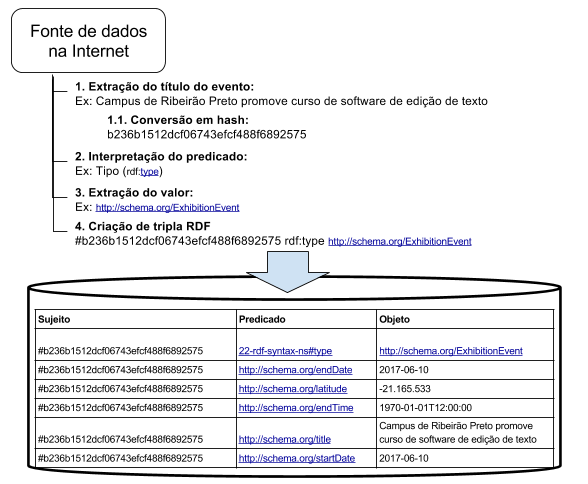
\includegraphics[width=.85\textwidth]{processo_geracao_triplas_rdf} 
  \caption{Processo de extração e conversão em triplas RDF}
  \label{fig:processo_geracao_triplas_rdf} 
\end{figure}

A biblioteca Jena permite armazenar e consultar triplas em RDF. No entanto uma propriedade torna esta biblioteca mais especial: a capacidade de realizar inferências sobre os próprios dados. Essa condição permite a realização de consultas que percorrem a estrutura de conceitos relacionada a um dado conceito alvo que oferece um resultado final mais rico, uma vez que inferem-se informações que antes não existiriam sem esse processo. A biblioteca TDB vai além, permitindo também a adição de novas regras que possam tornar o modelo ainda mais completo.

A capacidade de inferência da biblioteca Jena se dá por meio dos motores de inferência. Ela conta com motores pré-definidos que incluem um raciocinador transitivo que implementa apenas as propriedades transitivas e reflexivas da ontologia, um raciocinador RDF que implementa um subconjunto de implicações do RDF, um raciocinador OWL, OWL Mini, OWL Micro Reasoners que implementa um subconjunto de implicações do OWL/Lite e OWL/FULL e o raciocinador genérico baseado em regras defindas pelo usuário. Neste trabalho foram utilizados os raciocionadores RDF e Genérico para derivar informações a partir dos dados recuperados nos portais selecionados.

A camada de apresentação é o último sistema implementado neste trabalho e apresenta uma interface de pesquisa e exposição de informação que facilita a interação do usuário com a camada de persistência de dados, através da qual ele ira extrair informações relevantes. Esse objetivo foi alcançado por meio de uma área na qual as consultas são realizadas e os resultados são colocados em um mapa, conforme ilustrado pelo exemplo de uma consulta das estações de metrô em São Paulo ilustrado pela Figura~\ref{fig:integraweb_estacoes_metro}. Desse modo o sistema alterna entre consulta e apresentação de dados.

A consulta de dados no sistema acontece pela interação do usuário com as opções de consultas disponíveis na área 1 ilustrada na Figura~\ref{fig:mantichub_sistema}. Através dela é possível realizar diversos tipos de consultas, tanto as voltadas para usuários que não possuem domínio da linguagem SPARQL e que podem utilizar as pesquisas  pré-definidas por tipos de eventos, i.e, eventos em teatros, exposições, restaurantes entre outros quinze diferentes tipos de consultas pré-definidas utilizando a seleção ilustrada na área 2 ou, para usuários mais experientes, inserir a consulta SPARQL diretamente utilizando o campo de texto logo abaixo dessa área. Enquanto no primeiro caso a consulta por tipo de estabelecimento gera uma consulta SPARQL e depois é enviada para a camada de persistência, na segunda opção a consulta elaborada pelo usuário pula essa etapa e vai diretamente para a camada de persistência de dados. O resultado encontrado é então desenhado no mapa. Por fim, toda a consulta construída pode ser recuperada a qualquer momento clicando no botão ``Q'' (apresentado na área 3, no canto superior direito da tela). Ao clicar nesse botão, a consulta SPARQL que foi gerada no sistema é mostrada conforme apresentado na área 4 da interface.

\begin{figure}[!ht]
  \centering
  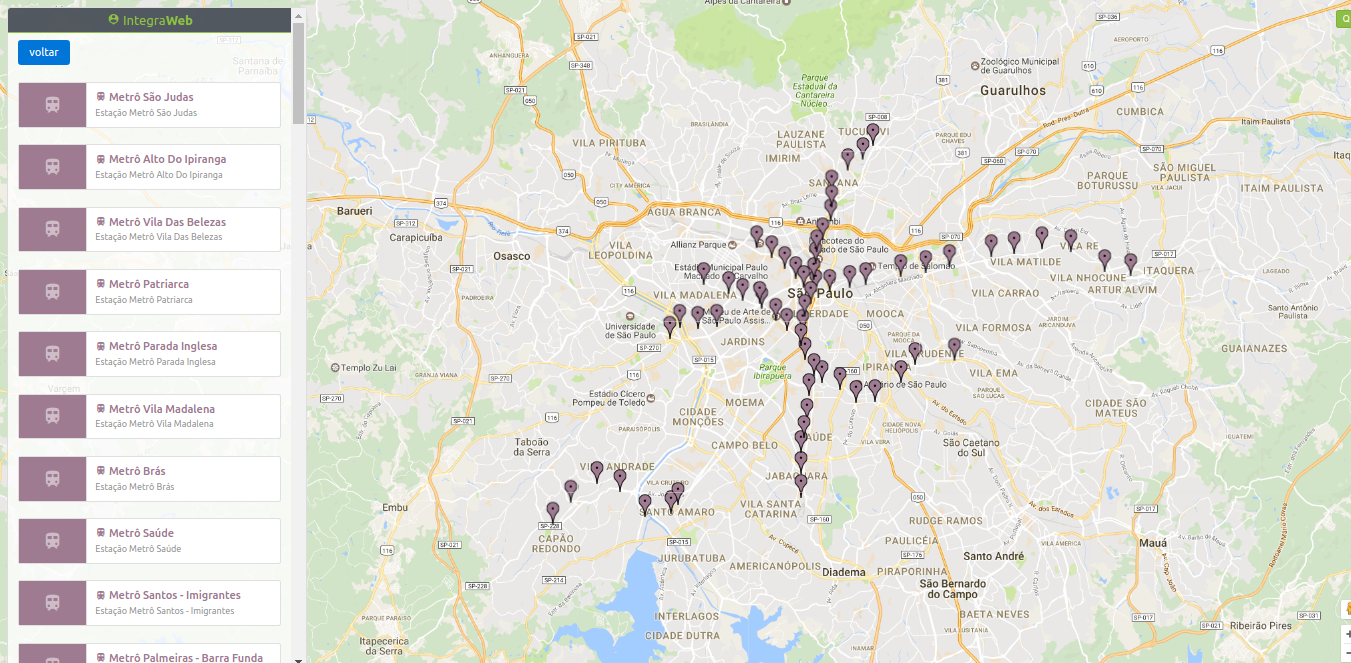
\includegraphics[width=.85\textwidth]{integraweb_estacoes_metro_2} 
  \caption{Estações de metrô em São Paulo}
  \label{fig:integraweb_estacoes_metro} 
\end{figure}

\begin{figure}[!ht]
  \centering
  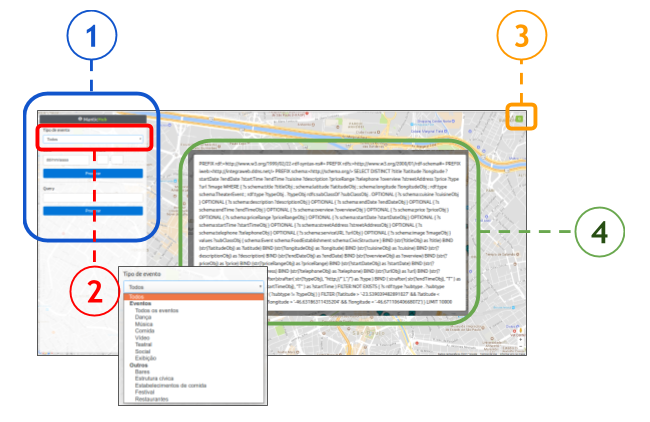
\includegraphics[width=.85\textwidth]{mantichub_estrutura_pesquisa} 
  \caption{Camada de apresentação da proposta}
  \label{fig:mantichub_sistema} 
\end{figure}


O resultado obtido a partir de uma interação de um usuário com a camada de apresentação é representado como um conjunto de pontos no mapa, e também como uma listagem no canto esquerdo da tela conforme ilustrado na Figura~\ref{fig:resultado_sistema_manticweb} nas áreas 1 e 2. Ao clicar em um desses pontos, é possível buscar mais detalhes sobre aquele estabelecimento especifico. Além disso, cada item possui uma marcação específica indicando a proveniência da informação, isso é, de qual portal entre os escolhidos ela foi obtida conforme ilustra a área 3; ao clica-los, é possível obter mais informações tais como data e hora, endereço, telefone, preço, link do site do qual a informação foi recuperada, entre outros. Por fim, é possível obter a consulta SPARQL gerada pelo sistema ao clicar no botão ``Q'' localizado na área 4.

\begin{figure}[!ht]
  \centering
  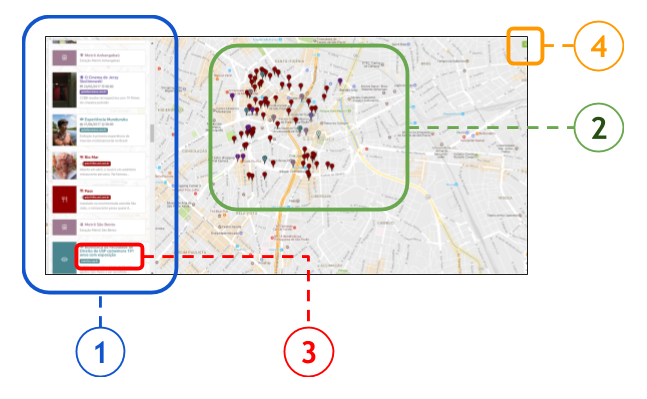
\includegraphics[width=.85\textwidth]{resultado_sistema_manticweb} 
  \caption{Interface de apresentação do resultado da consulta}
  \label{fig:resultado_sistema_manticweb} 
\end{figure}

Por fim, a implementação da arquitetura proposta esta disponível ao público na Internet no endereço ``http://integraweb.ddns.net''. Nesse portal, é possível interagir com o sistema a partir da base de dados que foi utilizada para a avaliação dos resultados neste trabalho, utilizando as consultas exemplos ou criando novas. Além disso, todo o código-fonte produzido também está exposto e pode ser acessado, analisado e carregado através do portal GitHub no endereço ``https://github.com/fpierin/mantichub''. A partir do conteúdo do repositório, é possível propor modificações na estrutura do projeto ou tomá-lo como base para novas implementações.

\section{Experimento 1: Integração de dados}
\label{sec:experimento_integracao_heterogenea}

Um primeiro experimento foi realizado de modo a ilustrar a integração de dados provenientes de fontes heterogêneas de informação. A Figura~\ref{fig:mantic_eventos_usp} mostra todos os eventos recuperados do portal Eventos USP. Nessa figura, é possível observar que esses eventos estão concentrados em regiões próximas a um campus da USP, como na região do Butantã, São Carlos ou Ribeirão Preto. Na Figura~\ref{fig:mantichub_eventos_guia_da_semana} vemos que os eventos recuperados pelo portal Guia Da Semana estão aglomerados na região central da cidade de São Paulo e abrangem em sua maioria peças de teatro, exposições ou shows. Já o Guia da Folha possui uma base de conteúdo mais diversificado e cobre praticamente toda a cidade de São Paulo, com informações sobre restaurantes, peças de teatro, exposições e bares como é possível observar na Figura~\ref{fig:mantichub_eventos_guia_da_folha}. 

Como neste trabalho todo o conteúdo dos portais citados foi recuperado e centralizado em um única base de dados, é possível realizar consultas  sem que o usuário tenha de consultar cada um dos portais individualmente, minimizando o seu trabalho manual de busca e provendo resultados mais abrangentes. 
 
\begin{figure}[!ht]
  \centering
  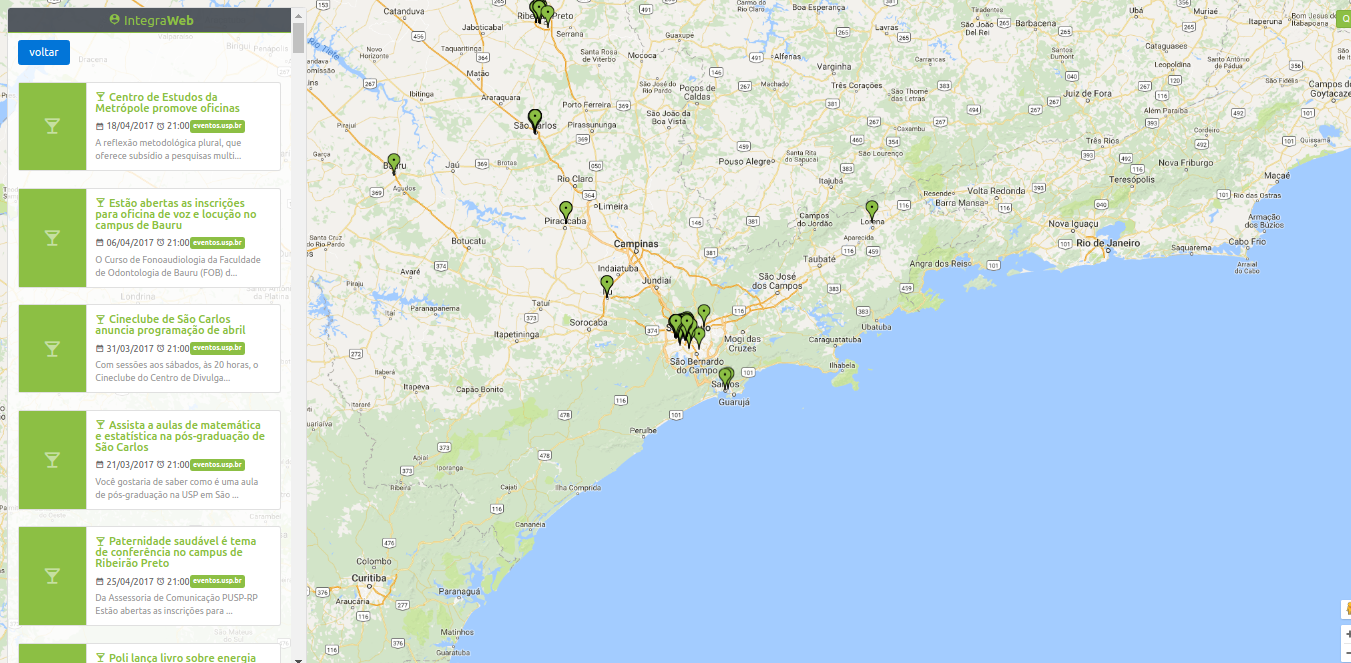
\includegraphics[width=.85\textwidth]{mantic_eventos_usp} 
  \caption{Concentração de dados do portal Eventos USP}
  \label{fig:mantic_eventos_usp} 
\end{figure}

\begin{figure}[!ht]
  \centering
  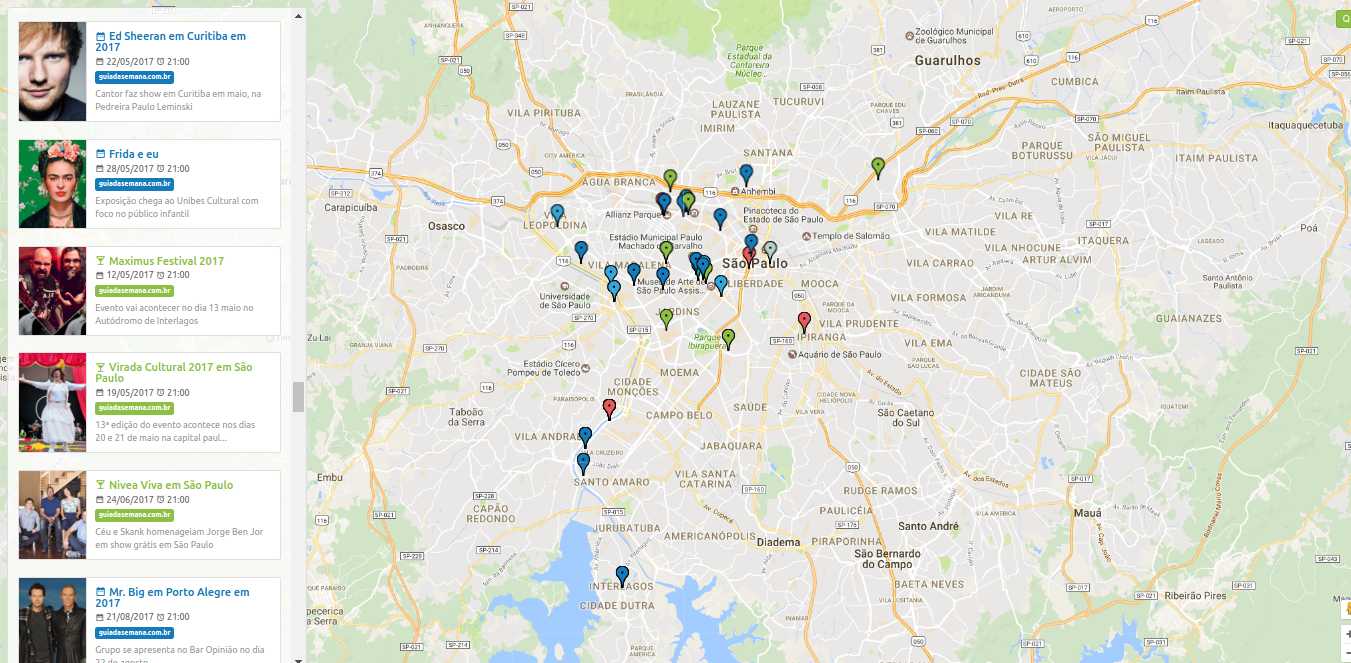
\includegraphics[width=.85\textwidth]{mantichub_eventos_guia_da_semana} 
  \caption{Concentração de dados do portal Guia da Semana}
  \label{fig:mantichub_eventos_guia_da_semana} 
\end{figure}

\begin{figure}[!ht]
  \centering
  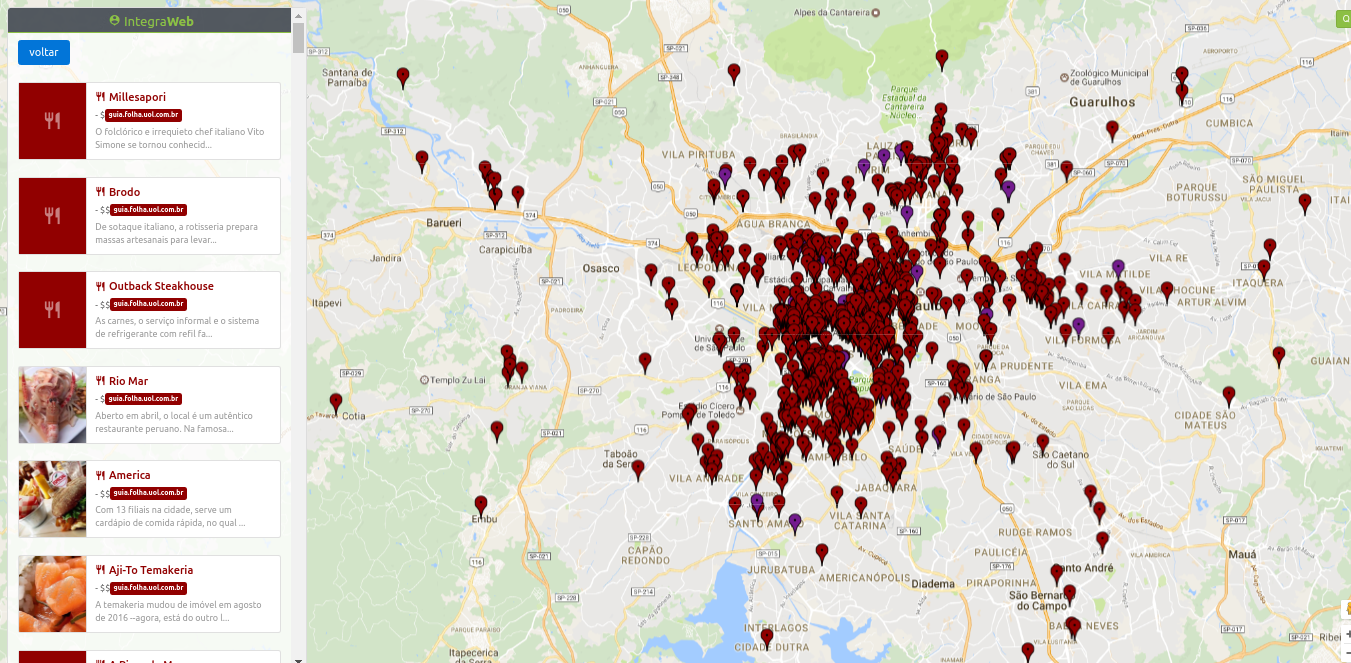
\includegraphics[width=.85\textwidth]{mantichub_eventos_guia_da_folha} 
  \caption{Concentração de dados do portal Guia da Folha}
  \label{fig:mantichub_eventos_guia_da_folha} 
\end{figure}

A busca de informações sobre eventos que ocorrem em uma determinada região da cidade tende a ser relevante para um individuo. Desse modo, para alcançar resultados sobre uma determinada região, é necessário saber os valores de latitude e longitude de um determinado ponto. Tomando como base o marco zero da cidade de São Paulo, situado na região da Praça da Sé, podem-se recuperar informações sobre eventos que ocorre num raio pré-definido com centro nessa região, por exemplo a 1km. Desse modo, utilizando a consulta SPARQL apresentada no anexo~\ref{ape:sparql-marco-zero} alcançamos o resultado apresentado na Figura~\ref{fig:mantichub_resultados_na_regiao}, que mostra restaurantes recuperados do portal Guia da Folha, eventos culturais dos portais Eventos USP e Guia da Semana e também algumas estações de Metrô que foram adicionadas à mesma base de dados.

\begin{figure}[!ht]
  \centering
  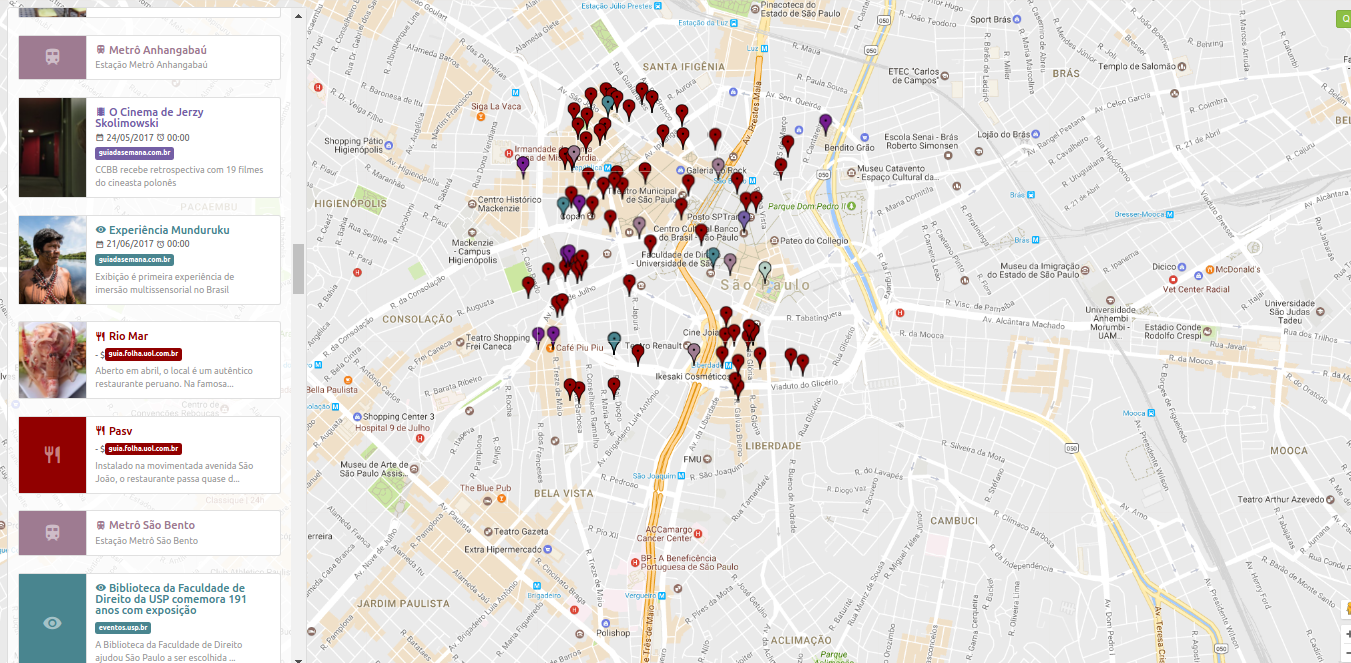
\includegraphics[width=.85\textwidth]{mantichub_resultados_na_regiao} 
  \caption{Concentração de eventos próximos ao Marco Zero de São Paulo}
  \label{fig:mantichub_resultados_na_regiao} 
\end{figure}

Neste exemplo, não ocorre duplicação ou conflito na integração dos dados. Em outras palavras, a informação sobre eventos e estabelecimentos que foi recuperada em um portal é complementar ao outro. A Figura~\ref{fig:sparql_portais} apresenta uma simplificação da consulta apresentada no Anexo~\ref{ape:sparql-marco-zero}.  Essa consulta retorna apenas o identificador do evento, o seu titulo e a origem dos dados. O resultado da consulta  encontra-se representado na Figura~\ref{fig:persistencia_dados_diferentes_portais}. Nesta figura, destacam-se os dados que são armazenados em cada uma das consultas aos diferentes portais.


\begin{figure}[!ht]
    \begin{lstlisting}[language=SPARQL]
PREFIX rdf:<http://www.w3.org/1999/02/22-rdf-syntax-ns#>
PREFIX rdfs:<http://www.w3.org/2000/01/rdf-schema#>
PREFIX schema:<http://schema.org/>
SELECT DISTINCT ?s ?title ?url
WHERE {
	?s schema:title ?titleObj ;
	schema:latitude ?latitudeObj ;
	schema:longitude ?longitudeObj ;
	rdf:type ?typeObj .
	?typeObj rdfs:subClassOf ?subClassObj .
	OPTIONAL { ?s schema:serviceURL ?urlObj }
	values ?subClassObj { schema:Event schema:FoodEstablishment schema:CivicStructure } 
	BIND (str(?titleObj) as ?title)
	BIND (str(?latitudeObj) as ?latitude)
	BIND (str(?longitudeObj) as ?longitude)
	BIND (str(?urlObj) as ?url)
	FILTER (?latitude > '-23.539606783940812' && ?latitude < '-23.55759321605919')
	FILTER (?longitude > '-46.62938980581791' && ?longitude < '-46.6490101941821')
	FILTER NOT EXISTS {
		?s rdf:type ?subtype .
		?subtype rdfs:subClassOf* ?typeObj .
		filter ( ?subtype != ?typeObj )
	}
 }
LIMIT 100
    \end{lstlisting}
    \caption{Consulta SPARQL para recuperar eventos próximos ao Marco Zero de São Paulo}
    \label{fig:sparql_portais} 
\end{figure}

Supondo que a recuperação dos dados aconteça primeiro no portal de Eventos da USP, a consulta retorna apenas dois eventos: a ``Comemoração da Faculdade de Direito'' e a ``Exposição no Centro de Preservação Cultural''. Se o sistema então obtiver os dados do portal Guia da Semana, novos eventos são adicionados, entre eles o musical ``Lès Miserables''. Finalmente, após o sistema recuperar o conteúdo do Portal Guia da Folha, outros eventos são acrescentados como, por exemplo, o evento ``A Experiência Munduruku''. Nesse contexto, a implementação da arquitetura conseguiu integrar os dados dos diferentes portais em uma única base de informações.

\begin{figure}[!ht]
  \centering
  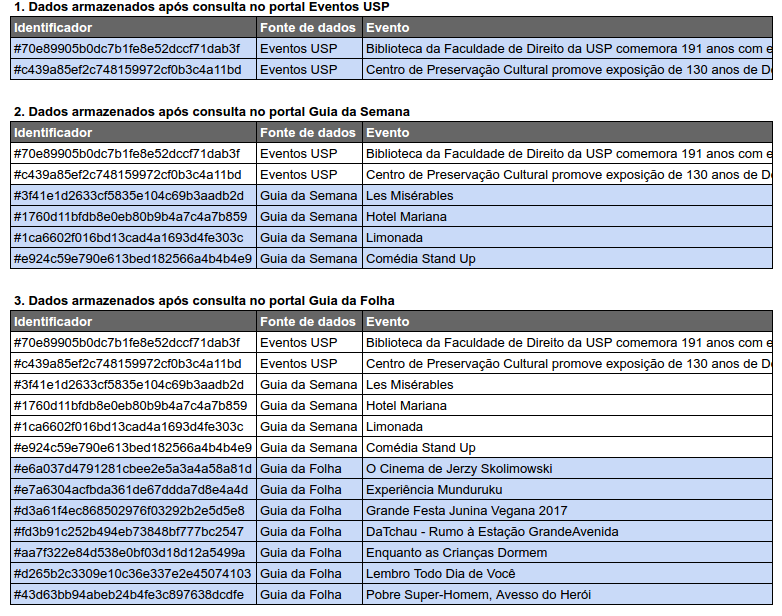
\includegraphics[width=.85\textwidth]{persistencia_dados_diferentes_portais} 
  \caption{Resultado do armazenamento de dados provenientes de diferentes portais}
  \label{fig:persistencia_dados_diferentes_portais} 
\end{figure}

\section{Experimento 2: Resolução de conflitos}
\label{sec:resolucao_de_conflitos_mesmo_evento}

A resolução de conflitos é uma tarefa essencial quando estamos lidando com informações provenientes de diferentes fontes de dados. Como conteúdos podem estar registrados de formas distintas nas diferentes fontes de informação, conflitos de informação podem ocorrer, e o contexto de eventos culturais não foge dessa situação. Por exemplo, uma  peça que acontece em um determinado teatro pode ter informações sobre preços, localização ou mesmo uma descrição totalmente diferentes em  fonte de dados distintas. Isso evidencia ser necessário um mecanismo capaz de resolver essas situações.

\begin{figure}[!ht]
\centering
  \begin{minipage}{.45\linewidth}
    \centering
    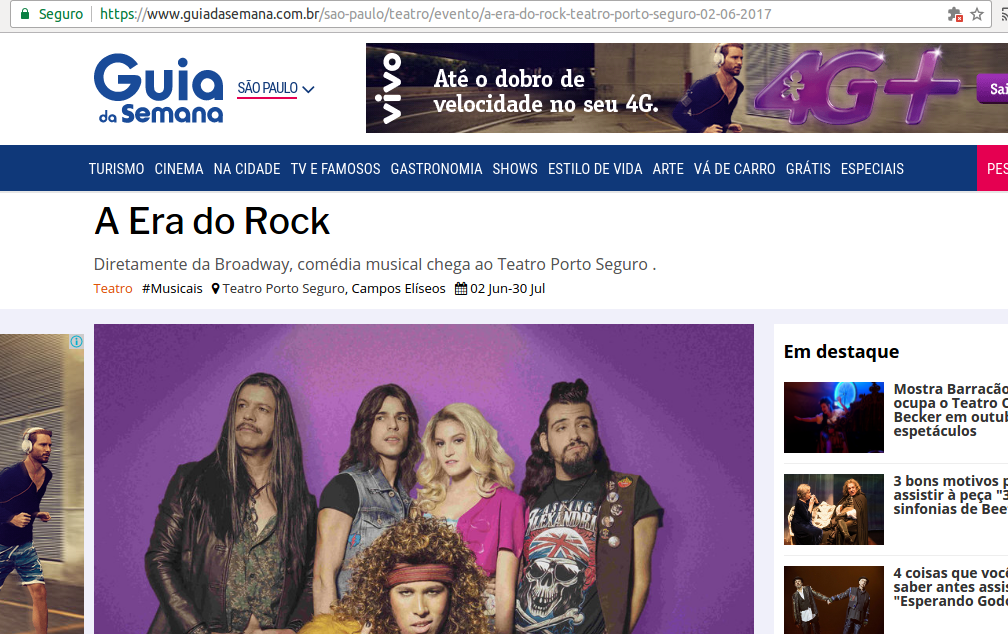
\includegraphics[width=0.85\textwidth]{a_era_do_rock} 
    \label{fig:a_era_do_rock}
  \end{minipage}
  \begin{minipage}{.45\linewidth}
    \centering
    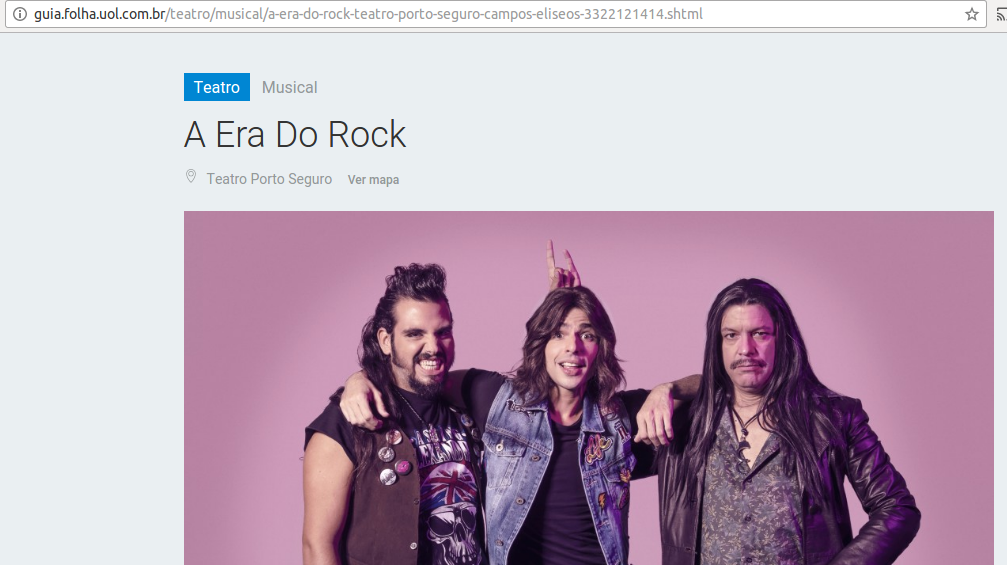
\includegraphics[width=0.95\textwidth]{a_era_do_rock_guia_folha}
    \label{fig:a_era_do_rock_guia_folha}
  \end{minipage}
  \caption{Evento "A Era do Rock" em diferentes portais}
  \label{fig:era_do_rock_dois_portais}
\end{figure}

\begin{figure}[!ht]
  \centering
  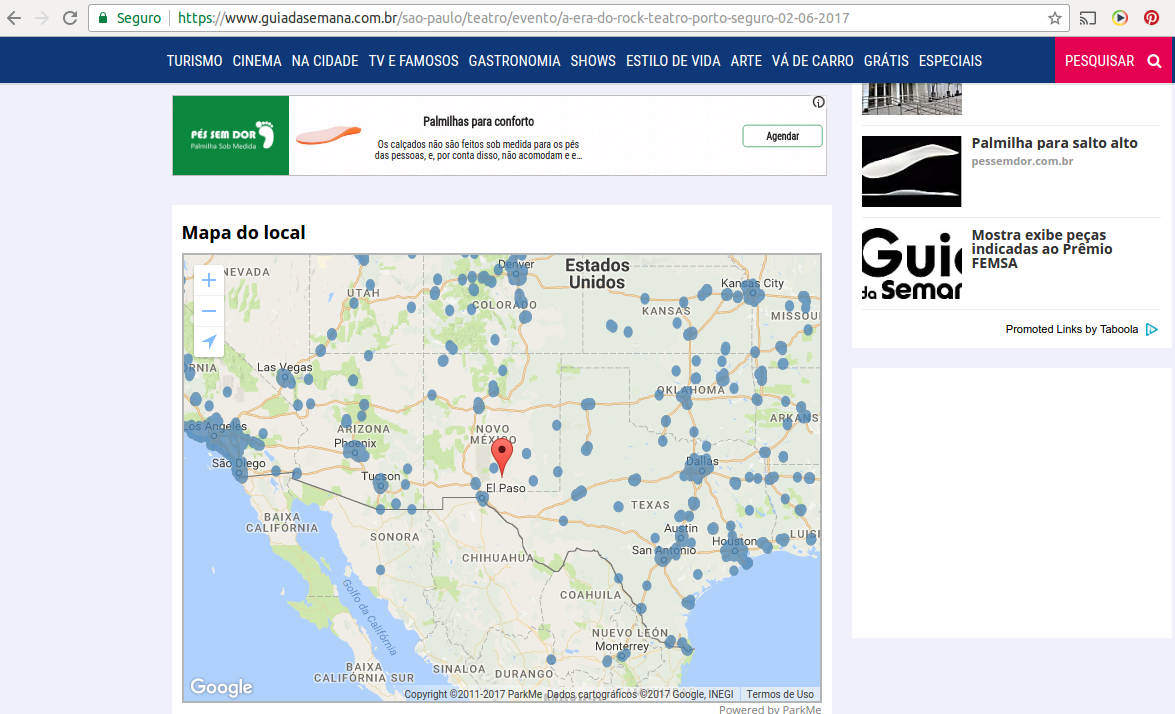
\includegraphics[width=.85\textwidth]{localizacao_incorreta_a_era_do_rock} 
  \caption{Geolocalização de evento incorreta no portal Guia da Semana}
  \label{fig:localizacao_incorreta_a_era_do_rock} 
\end{figure}

\begin{figure}[!ht]
  \centering
  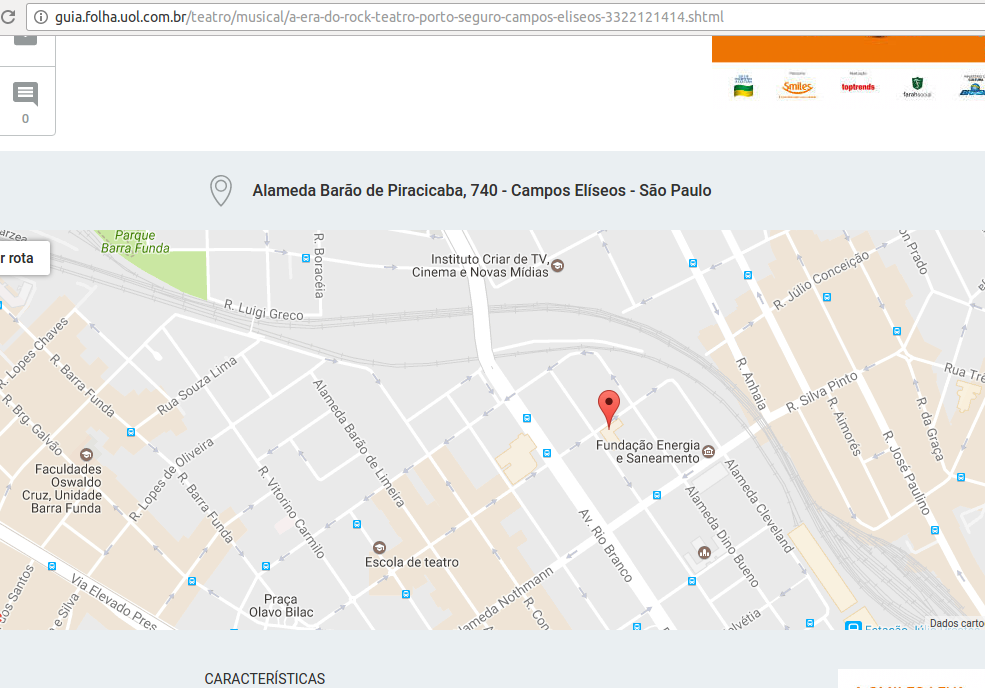
\includegraphics[width=.85\textwidth]{localizacao_correta_guia_da_folha} 
  \caption{Geolocalização de evento correta no portal Guia da Folha}
  \label{fig:localizacao_correta_guia_da_folha} 
\end{figure}

No modelo proposto neste neste trabalho, há uma hierarquia de preferência da informação. Desse modo, uma fonte de dados por ser mais confiável que as outras sempre terá preferência em relação a sua informação. Um exemplo desta situação se refere à peça de teatro ``A Era do Rock'',  que aparece tanto no portal Guia da Folha quanto no portal Guia da Semana, como mostra a Figura~\ref{fig:era_do_rock_dois_portais}. Embora a informação sobre um mesmo evento seja exibida em ambos os portais de eventos, a extração de dados de uma determinada fonte pode ser mais consistente do que outra por motivos diversos que vão desde a quantidade de revisores de conteúdo, investimento a quantidade de atualizações. Nesse caso específico, a informação sobre geolocalização do evento está incorreta no Guia da Semana e correta no Guia da Folha. Enquanto na primeira fonte de dados marca  um local de exibição fora do pais e claramente incorreto, conforme ilustra a Figura~\ref{fig:localizacao_incorreta_a_era_do_rock}, no segundo a informação marca corretamente o Teatro Porto Seguro, conforme ilustra a Figura~\ref{fig:localizacao_correta_guia_da_folha}. Quando a informação é recuperada do portal Guia da Folha e adicionada ao sistema, como o portal Guia da Folha possui preferência sobre a informação do site Guia da Semana, a geolocalização incorreta é então substituída e a informação torna-se mais confiável.

A consulta SPARQL, ilustrada na Figura~\ref{fig:sparql_era_do_rock}, permite observar como os dados são armazenados e modificados conforme a informação é recuperada na Internet. A Figura~\ref{fig:guia_da_semana_antes} é um exemplo de quando os dados do evento são capturados de uma fonte de dados com inconsistência da informação e adicionados à base de conhecimento. A Figura~\ref{fig:guia_da_semana_depois} representa os dados ajustados após o processo de resolução de conflitos por fonte mais confiável. Outra vantagem da proposta apresentada neste trabalho é a capacidade de combinar as informações provenientes das diferentes fontes escolhidas. No exemplo anterior, além de atualizar a informação sobre latitude e longitude do evento, a informação também foi complementada com uma descrição mais específica com o título "overview" o que agrega mais detalhes e consequentemente oferece uma informação mais abrangente ao usuário final.

\begin{figure}[!htbp]
    \begin{lstlisting}[language=SPARQL]
PREFIX rdf:<http://www.w3.org/1999/02/22-rdf-syntax-ns#>
PREFIX rdfs:<http://www.w3.org/2000/01/rdf-schema#>
PREFIX iweb:<http://integraweb.ddns.net/>
PREFIX schema:<http://schema.org/>
SELECT DISTINCT ?s ?title ?latitude ?longitude ?startDate ?endDate ?startTime ?endTime ?cuisine ?description ?priceRange ?telephone ?overview ?streetAddress ?price ?type ?url ?image 
WHERE {
	?s schema:title ?titleObj ;
	schema:latitude ?latitudeObj ;
	schema:longitude ?longitudeObj ;
	rdf:type schema:TheaterEvent ;
	rdf:type ?typeObj .
	?typeObj rdfs:subClassOf ?subClassObj .
	OPTIONAL { ?s schema:cuisine ?cuisineObj }
	OPTIONAL { ?s schema:description ?descriptionObj }
	OPTIONAL { ?s schema:endDate ?endDateObj }
	OPTIONAL { ?s schema:endTime ?endTimeObj }	
	OPTIONAL { ?s schema:overview ?overviewObj }
	OPTIONAL { ?s schema:price ?priceObj }	
	OPTIONAL { ?s schema:priceRange ?priceRangeObj }
	OPTIONAL { ?s schema:startDate ?startDateObj }
	OPTIONAL { ?s schema:startTime ?startTimeObj }
	OPTIONAL { ?s schema:streetAddress ?streetAddressObj }	
	OPTIONAL { ?s schema:telephone ?telephoneObj }
	OPTIONAL { ?s schema:serviceURL ?urlObj }
	OPTIONAL { ?s schema:image ?imageObj }
	values ?subClassObj { schema:Event schema:FoodEstablishment schema:CivicStructure } 
	BIND (str(?titleObj) as ?title)
	BIND (str(?latitudeObj) as ?latitude)
	BIND (str(?longitudeObj) as ?longitude)
	BIND (str(?cuisineObj) as ?cuisine)
	BIND (str(?descriptionObj) as ?description)
	BIND (str(?endDateObj) as ?endDate)
	BIND (str(?overviewObj) as ?overview)
	BIND (str(?priceObj) as ?price)
	BIND (str(?priceRangeObj) as ?priceRange)
	BIND (str(?startDateObj) as ?startDate)
	BIND (str(?streetAddressObj) as ?streetAddress)
	BIND (str(?telephoneObj) as ?telephone)
	BIND (str(?urlObj) as ?url)
	BIND (str(?imageObj) as ?image)
	BIND ( strafter(strafter( str(?typeObj), "http://" ),"/") as ?type )
	BIND ( strafter( str(?endTimeObj), "T" ) as ?endTime )
	BIND ( strafter( str(?startTimeObj), "T" ) as ?startTime )
	FILTER (?title = 'A Era do Rock')
	FILTER NOT EXISTS {
		?s rdf:type ?subtype .
		?subtype rdfs:subClassOf* ?typeObj .
		filter ( ?subtype != ?typeObj )
	}	
 }
LIMIT 100
    \end{lstlisting}
    \caption{Consulta sobre o evento "A Era do Rock"}
    \label{fig:sparql_era_do_rock} 
\end{figure}

\begin{figure}[!ht]
  \centering
  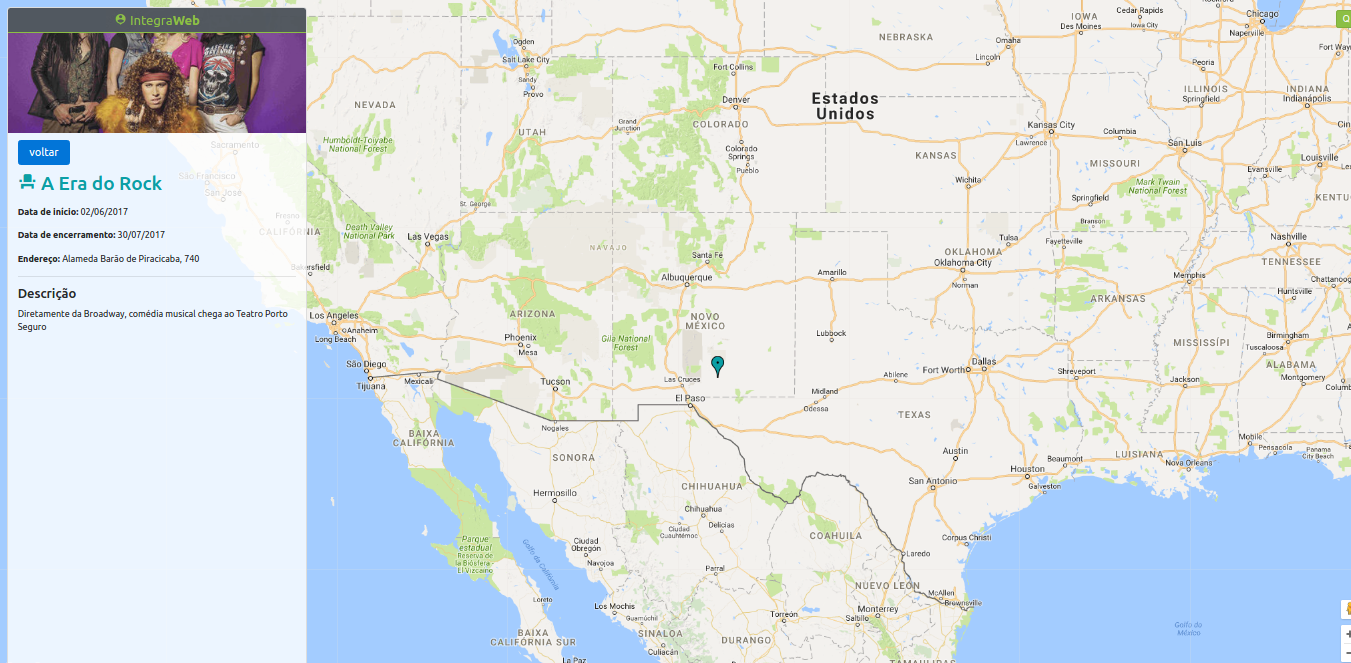
\includegraphics[width=.85\textwidth]{guia_da_semana_antes} 
  \caption{Informação inconsistente antes da resolução de conflitos}
  \label{fig:guia_da_semana_antes} 
\end{figure}

\begin{figure}[!ht]
  \centering
  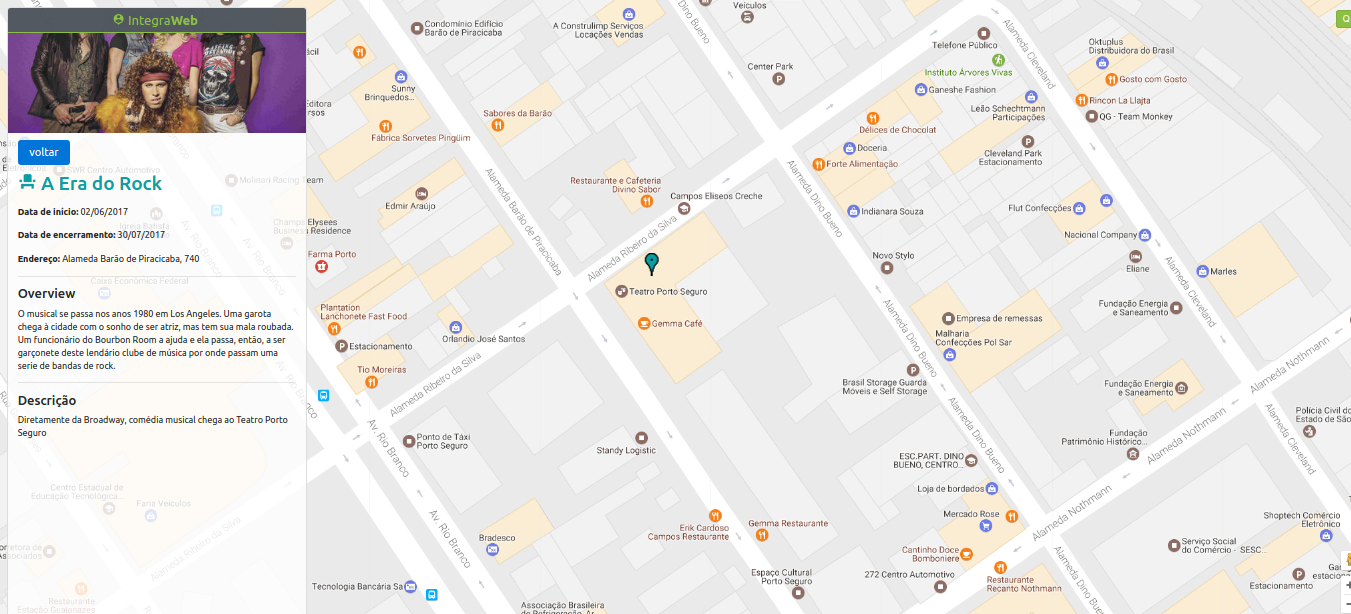
\includegraphics[width=.85\textwidth]{guia_da_semana_depois} 
  \caption{Informação consistente após resolução de conflitos}
  \label{fig:guia_da_semana_depois} 
\end{figure}

O processo de atualização da informação sobre o evento ``A Era do Rock'' pode ser observado também do ponto de vista da camada de persistência de dados, conforme ilustrado pela Figura~\ref{fig:tabela_valores}. Após a extração do conteúdo do portal Guia da Semana, várias triplas RDF foram geradas definindo propriedades como o titulo, latitude, longitude, descrição, endereço na Internet, entre outros. Nesse momento ainda não havia conteúdo sobre o evento na base de dados, e portanto todas as triplas foram persistidas. Na sequencia, a informação foi recuperada do portal Guia da Folha. Nesse momento, todas as propriedades encontradas no portal e que já estavam armazenadas na base de dados foram substituídas pelo valor encontrado, em especial os que estão marcados nas linhas em negrito com fundo amarelo: latitude, longitude, endereço do site e da imagem de referência. Além disso, a descrição que ainda não existia foi adicionada (propriedade ``overview'') e mesclada junto as outras propriedades do espetáculo, conforme destacado na linha destacada com fundo verde.

\begin{figure}[!ht]
  \centering
  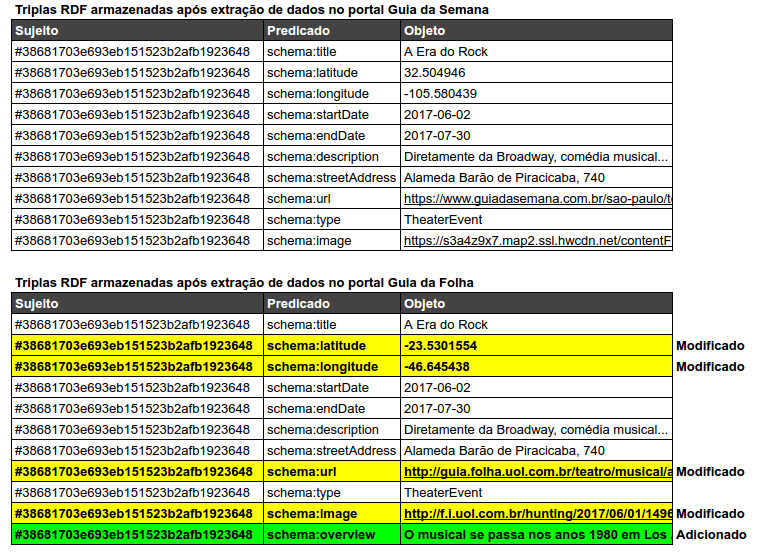
\includegraphics[width=.85\textwidth]{tabela_valores} 
  \caption{Dados obtidos após extração nos diferentes portais}
  \label{fig:tabela_valores} 
\end{figure}



\section{Experimento 3: Consultas combinadas entre diferentes conceitos}
\label{sec:combinacao_consultas}

A combinação de interesses é um dos objetivos mais interessantes para um usuário que realiza uma consulta a respeito de eventos. É bastante comum nos depararmos com situações em que desejamos ter uma visão ampla sobre os estabelecimentos de uma determinada região para que possa ser possível nos programar para alcançar diferentes finalidades pessoais. Um exemplo disso é quando queremos encontrar restaurantes próximos a um determinado evento do qual já sabemos com antecedência que iremos participar. A Figura~\ref{fig:restaurantes_perto_evento} mostra um exemplo em que temos a informação de todos os restaurantes próximos ao evento escolhido. Essa informação é um apoio a decisão final do usuário. Pode-se ir além e restringir ainda mais  essas opções, alterando a consulta para mostrar apenas os restaurantes que servem comida alemã, como mostra a Figura~\ref{fig:comida_alema_perto_evento}. 

\begin{figure}[!ht]
  \centering
  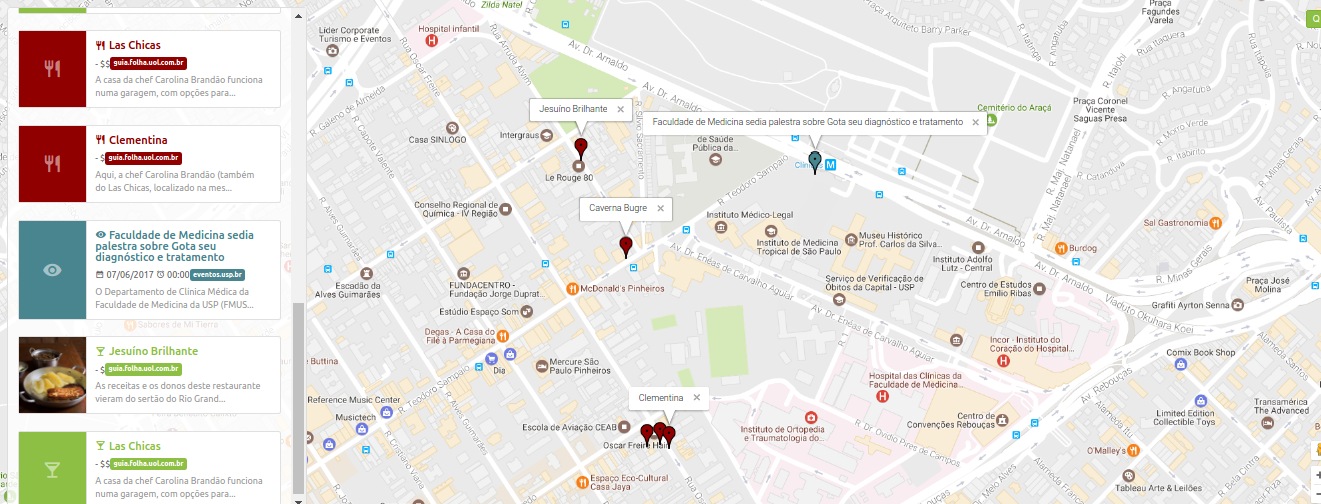
\includegraphics[width=.85\textwidth]{restaurantes_perto_evento} 
  \caption{Restaurantes próximo a um evento}
  \label{fig:restaurantes_perto_evento} 
\end{figure}

\begin{figure}[!ht]
  \centering
  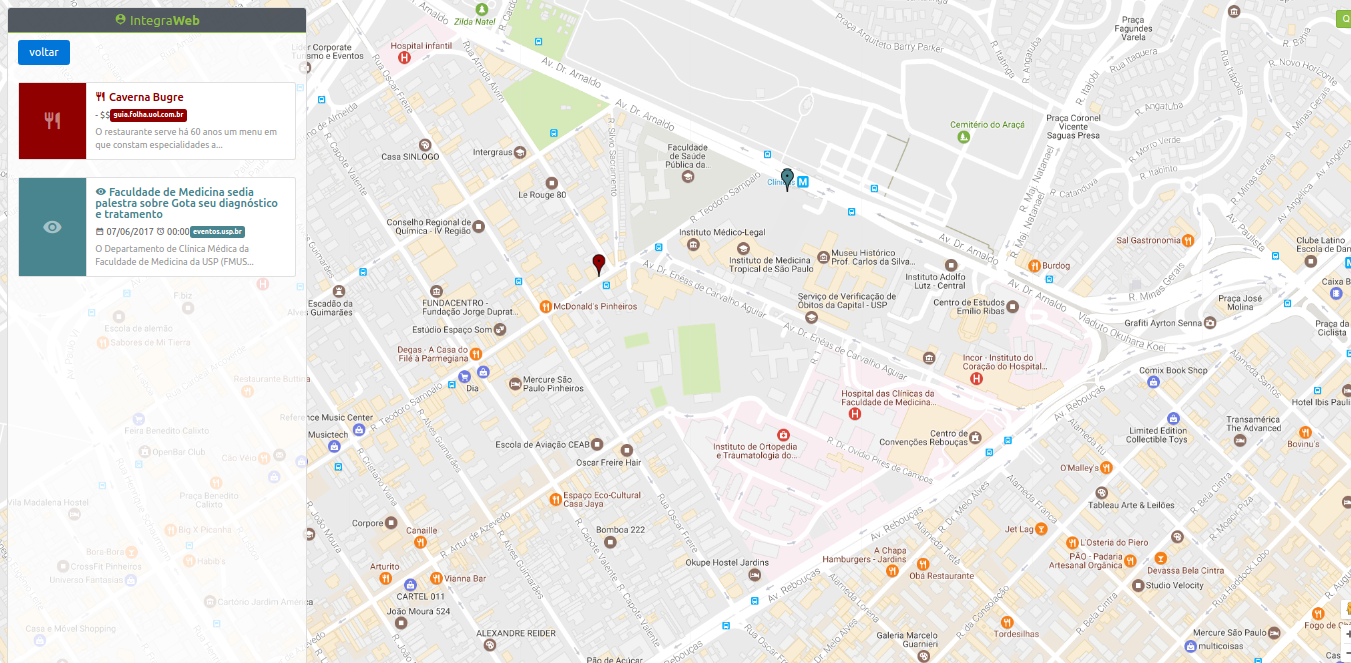
\includegraphics[width=.85\textwidth]{comida_alema_perto_evento} 
  \caption{Restaurantes de comida alemã próximo a um evento}
  \label{fig:comida_alema_perto_evento} 
\end{figure}

A partir dos dados centralizados em uma única base com informação semântica, aumenta-se as possibilidades de pesquisa de um usuário. Outro exemplo interessante concerne indivíduos que estão migrando para o transporte público e deixando de lado os seus carros. Para esse tipo de usuário, ter a informação sobre o que ocorre próximo ao metrô pode vir a definir a escolha de um evento em relação a outro. A Figura~\ref{fig:bares_proximo_ao_metro} mostra uma pesquisa por bares próximos ao metrô. Seguindo a ideia de restrição de consultas, é possível melhorar ainda mais a pesquisa e consultar, por exemplo, apenas os eventos que estão próximo a um metrô, por exemplo o da praça da Sé, como ilustra a Figura~\ref{fig:eventos_proximo_metro_se}.

\begin{figure}[!ht]
  \centering
  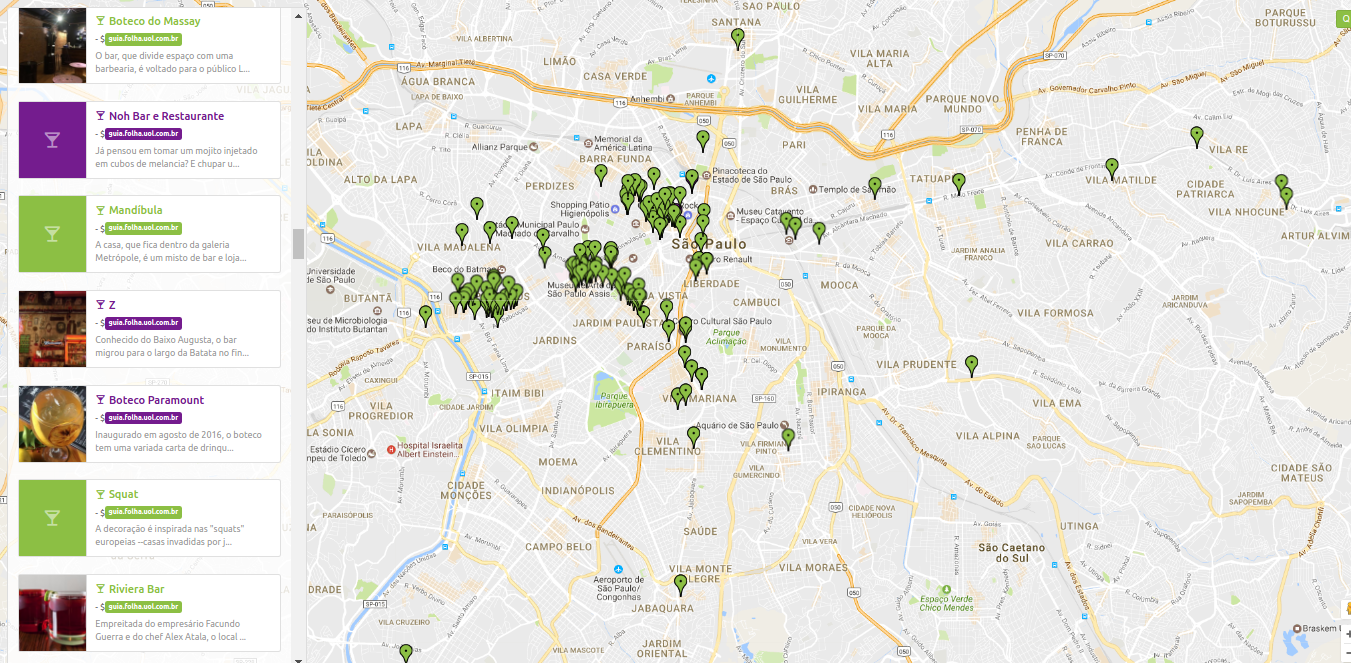
\includegraphics[width=.85\textwidth]{bares_proximo_ao_metro} 
  \caption{Bares próximos a estações de metrô}
  \label{fig:bares_proximo_ao_metro} 
\end{figure}

\begin{figure}[!ht]
  \centering
  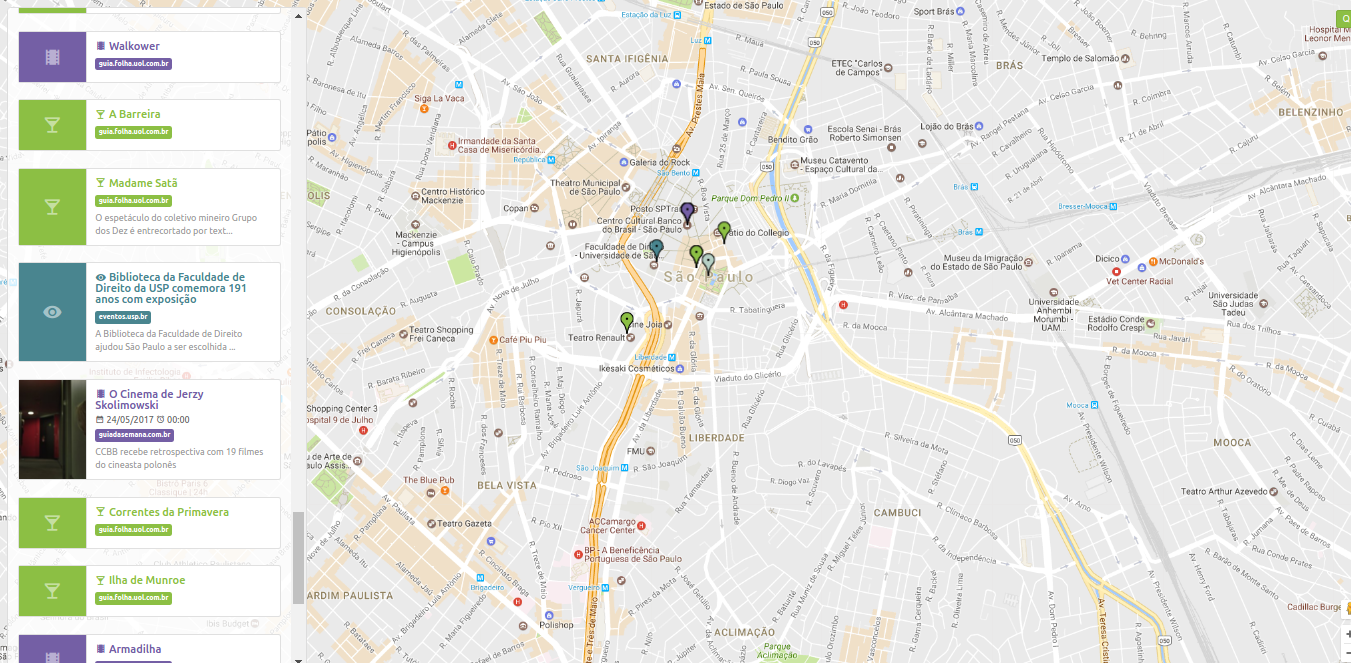
\includegraphics[width=.85\textwidth]{eventos_proximo_metro_se} 
  \caption{Bares próximos à estação de metrô Sé}
  \label{fig:eventos_proximo_metro_se} 
\end{figure}

A combinação de dados pode ser ainda mais complexa de maneira, a tornar possível programar uma agenda mais completa para o dia de uma pessoa. Suponha a situação em que um individuo que tenha interesse em conversar com um velho amigo em um bar, levar a esposa para a exposição ``Fiaminghi - Pensamentos Compostos'' e, por fim, fazer uma surpresa para ela levando-a para um restaurante de comida Natural. Para que o usuário aproveite melhor os momentos, é importante que os eventos estejam próximos uns dos outros para que ele possa se deslocar, andando sem se demorar. Nessa situação, a resposta pode ser obtida por uma consulta mais elaborada sobre a base de dados conforme o exemplo de código SPARQL resumido apresentado na Figura~\ref{fig:sparql_consultas_compostas}. Tal consulta retorna as informações  ilustradas na Figura~\ref{fig:combinacao_tres_eventos} e auxilia o usuário na tomada de decisão. A consulta completa pode ser encontrada no anexo~\ref{ape:consultas-varias-restricoes}.

\begin{figure}[!ht]
    \begin{lstlisting}[language=SPARQL]
...
PREFIX iweb:<http://integraweb.ddns.net/>
PREFIX schema:<http://schema.org/>
SELECT ?title ?latitude ?longitude ?startDate ?endDate ?startTime ?endTime ?cuisine ?description ?priceRange ?telephone ?overview ?streetAddress ?price ?type ?url ?image ?servesCuisine WHERE {
	{
		?s schema:title ?titleObj ;
		schema:latitude ?latitudeObj ;
		schema:longitude ?longitudeObj ;
		iweb:near ?nearObj ; 
		rdf:type schema:Restaurant ;
		schema:servesCuisine ?servesCuisineObj ;
		rdf:type ?typeObj .
		?nearObj schema:title ?nearObjTitle .
		...
    	FILTER (str(?nearObjTitle) = 'Fiaminghi - Pensamentos Compostos')
		FILTER (?servesCuisine = 'Natural')
		...
	}
	UNION 
	{
		...
		FILTER (?title = 'Fiaminghi - Pensamentos Compostos')
		FILTER (?type = 'ExhibitionEvent')
		...
	}
	UNION 
	{
		...
		iweb:near ?nearObj ; 
		rdf:type schema:BarOrPub ;
		...
		FILTER (str(?nearObjTitle) = 'Fiaminghi - Pensamentos Compostos')
		...
	}
}
    \end{lstlisting}
    \caption{Consulta relacionando estabelecimentos distintos}
    \label{fig:sparql_consultas_compostas} 
\end{figure}

\begin{figure}[!ht]
  \centering
  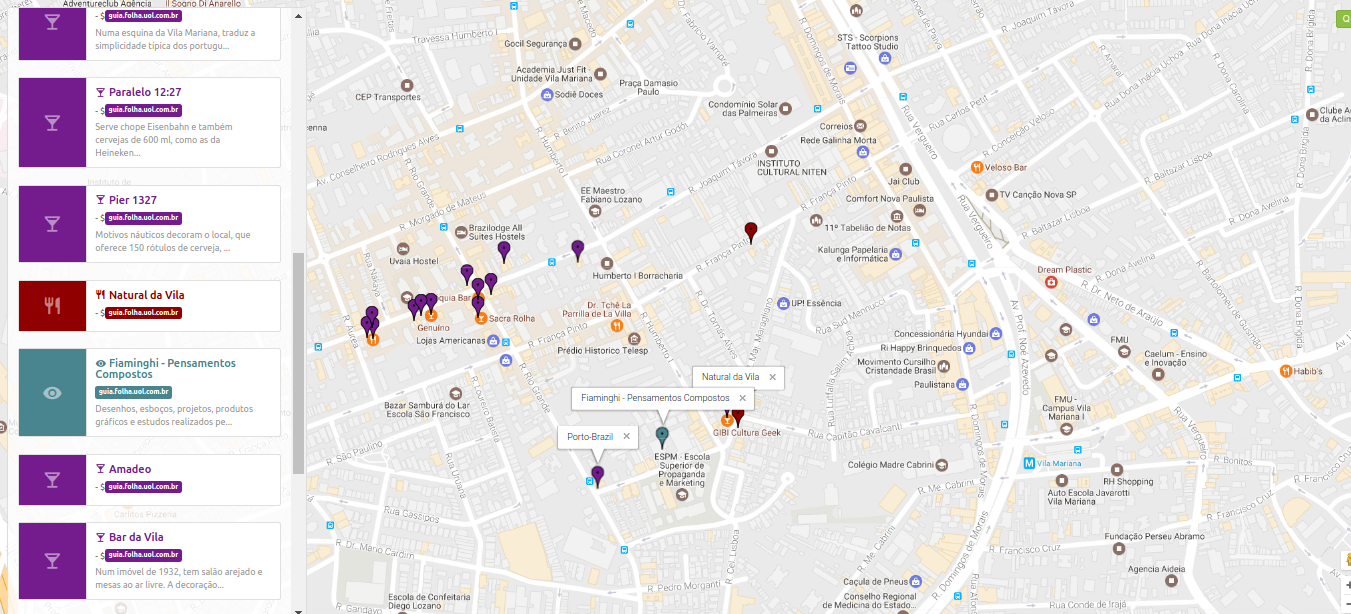
\includegraphics[width=.85\textwidth]{combinacao_top} 
  \caption{Busca por evento, bar e restaurante próximos}
  \label{fig:combinacao_tres_eventos} 
\end{figure}


O exemplo anterior demonstra que é possível realizar uma busca que integra a informação de diferentes conceitos: bares, eventos e restaurantes. No entanto, os dados apresentados eram todos do portal Guia da Folha. Ainda que seja custoso, avaliar os dados contidos dentro de um mesmo portal é mais fácil do que quando a informação está espalhada por diferentes portais  da Internet. Quanto mais informações precisam ser avaliadas e quanto mais portais precisam ser visitados, mais difícil é chegar a um resultado mais assertivo. A tarefa é ainda maior quando se é preciso avaliar a distância entre locais de diferentes eventos, quando cada um deles é retornado por um portal distinto. Apesar disso, quando a arquitetura proposta nesse trabalho é aplicada, essa tarefa torna-se trivial pois toda a informação está concentrada em um só banco. A Figura~\ref{fig:comida_coreana} exemplifica uma variação do exemplo anterior. Vamos agora levar em consideração o evento ``Metrópole: experiência paulista'' que está sendo divulgado apenas pelo portal de eventos da USP, bares e restaurante de comida coreana próximos. Verifica-se que a arquitetura consegue integrar a informação de diferentes portais e associá-la por meio de conceitos como bar, restaurante, tipo de comida, etc. Essa característica simplifica bastante a interação do usuário com as informações espalhadas na Internet.

\begin{figure}[!ht]
  \centering
  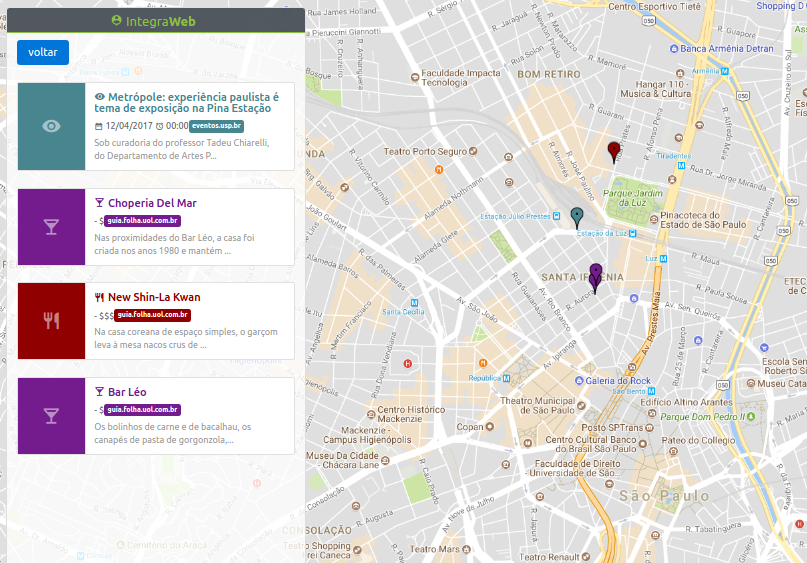
\includegraphics[width=.85\textwidth]{comida_coreana} 
  \caption{Busca integrando diferentes conceitos sobre dados de diferentes portais}
  \label{fig:comida_coreana} 
\end{figure}

